%%%%%%%%%%%%%%%%%%%%
%% PSCF program
%% ~Readme.tex~
%% $Rev$
%% Sept. 2009
%% Satoshi Takahama (stakahama@ucsd.edu)
%%%%%%%%%%%%%%%%%%%%

\documentclass{article}
\usepackage{texmf/Sweave}

\usepackage[usenames]{color}
\definecolor{darkred}{rgb}{0.545,0,0}
\definecolor{midnightblue}{rgb}{0.098,0.098,0.439}
\DefineVerbatimEnvironment{Sinput}{Verbatim}{fontshape=sl,
formatcom=\color{midnightblue}}
\DefineVerbatimEnvironment{Soutput}{Verbatim}{formatcom=\color{darkred}}
\DefineVerbatimEnvironment{Scode}{Verbatim}{fontshape=sl,
formatcom=\color{blue}}
\fvset{listparameters={\setlength{\topsep}{2pt}}} 
\renewenvironment{Schunk}{\vspace{\topsep}}{\vspace{\topsep}} 
\usepackage{fullpage}
\parindent 0in
\title{PSCF demo}
\date{}
\setkeys{Gin}{width=1.0\textwidth}
\begin{document}
\maketitle

\section{Preliminaries}

There are two steps for PSCF analysis:
\begin{enumerate}
\item Generate back-trajectories using HYSPLIT
\item Create a grid over your domain and overlay HYSPLIT
  backtrajectories for the PSCF analysis.
\end{enumerate}

Two important things to consider: 
\begin{enumerate}
\item Regarding trajectory generation: how often to generate, time
  resolution, how far back in time
\item For PSCF or density calculation: spacing of grid points, whether
  to count each point in trajectory or the trajectory itself which
  passes over a given grid cell.
\end{enumerate}

\section{Part 1: Running HYSPLIT}

Code diagram (note, \verb@demo.R@ may now be called \verb@PSCFdemo.R@):
\begin{center}
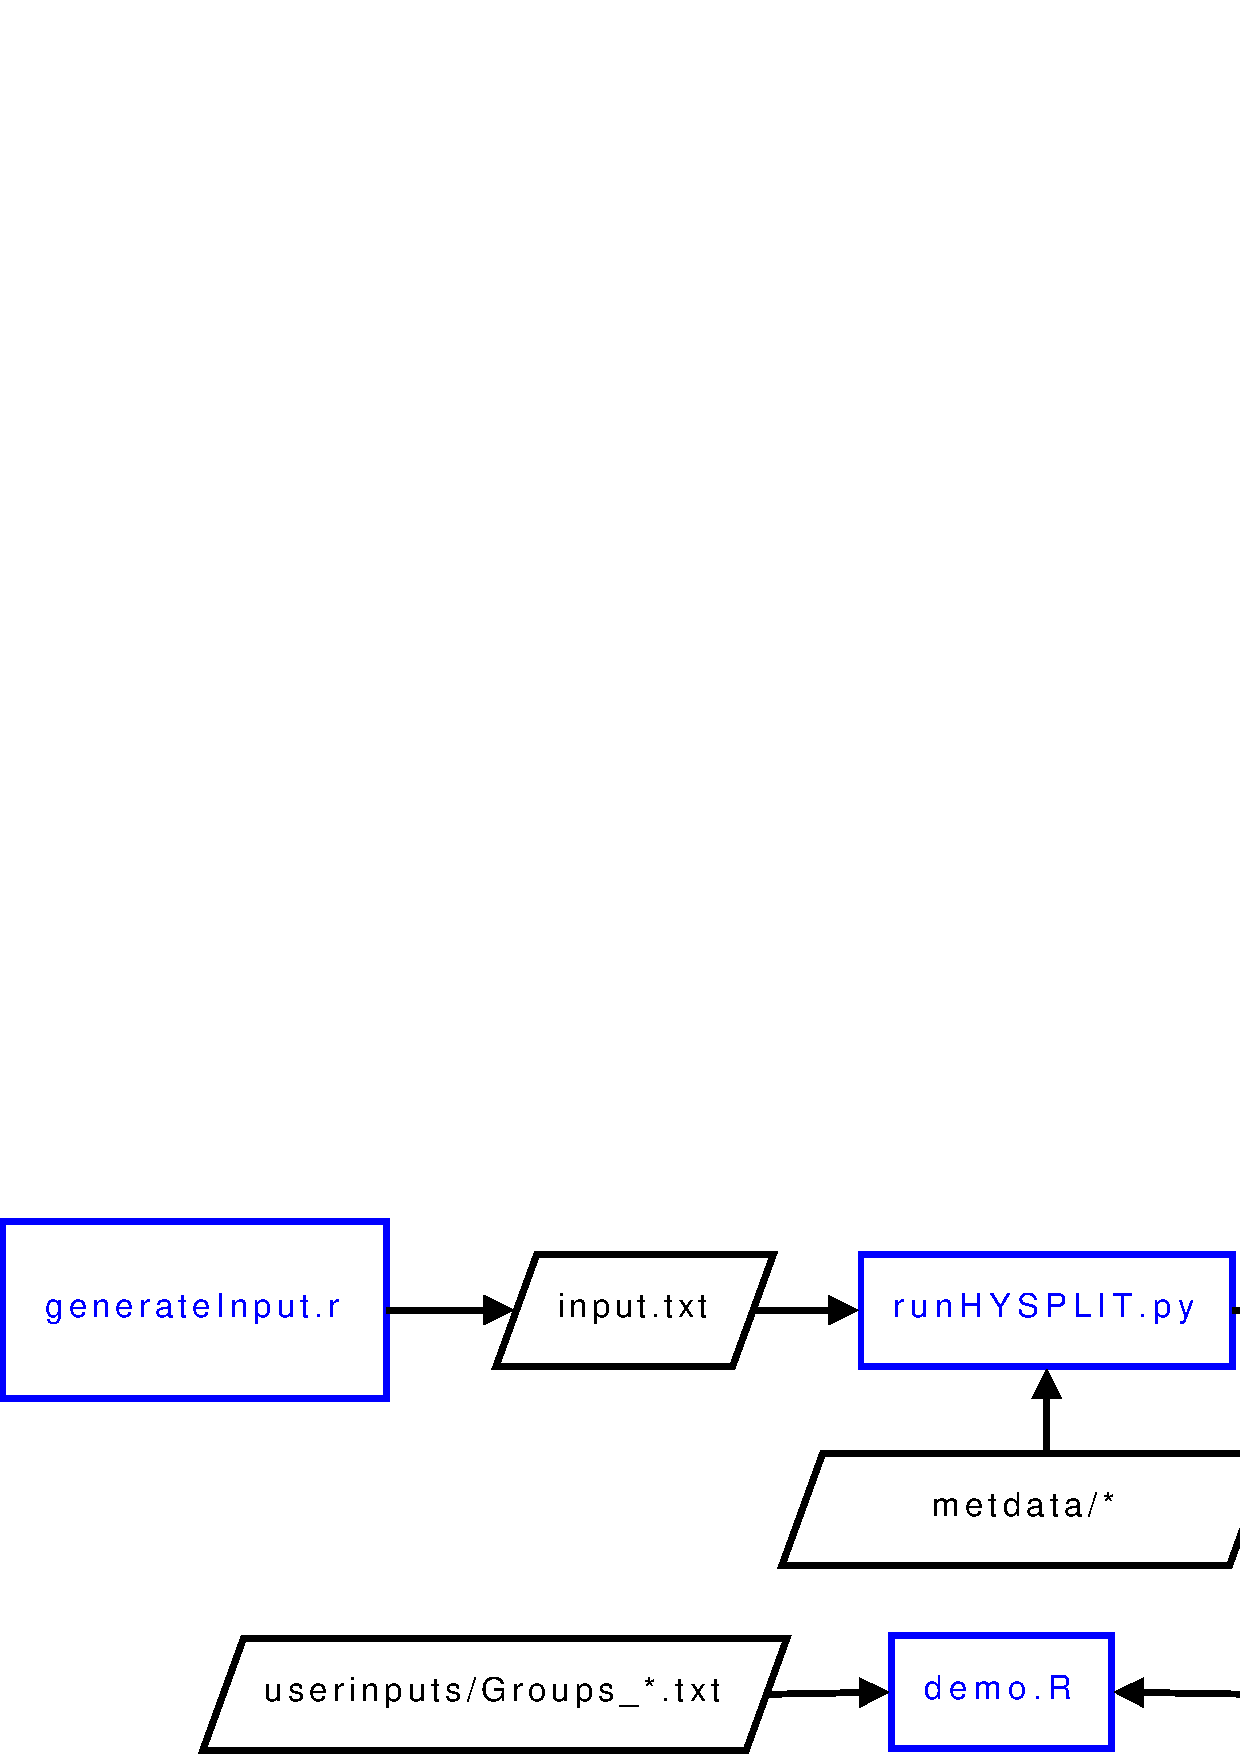
\includegraphics[width=.7\textwidth]{figures/IO.pdf}  
\end{center}

\begin{enumerate}
\item Download and place meteorological files in \verb@metdata/@.
\item Edit the desired conditions in \verb@generateInput.r@
\begin{Schunk}
\begin{Soutput}
## === user input ===
Start_lat <- 32.12
Start_lon <- -116.97
Start_alt <- c(1000,1200)
Start_times <- seq.chron(from=strptime2chron("4/25/09 00:00:00"),
                         to=strptime2chron("4/26/09 00:00:00"),
                         by=times("02:00:00"))
                                        # alternatively: by="hour"
                                        # and so on
Run_hours <- -5
Vert_coord <- 0
Model_top <- 1000000
\end{Soutput}
\end{Schunk}

This will generate a file called \verb@input.txt@ which is a table containing
the inputs (by row) for HYSPLIT. \verb@input.txt@ is a tab-delimited
file with the following format:
  
\begin{Schunk}
\begin{Soutput}
Latitude  Longitude  Altitude  Time  Run_hours  Vert_coord  Model_top
32.1200  -116.9700  1000.0000  04/25/09 00:00:00  -5  0  1000000.0000
32.1200  -116.9700  1200.0000  04/25/09 00:00:00  -5  0  1000000.0000
32.1200  -116.9700  1000.0000  04/25/09 02:00:00  -5  0  1000000.0000
32.1200  -116.9700  1200.0000  04/25/09 02:00:00  -5  0  1000000.0000
32.1200  -116.9700  1000.0000  04/25/09 04:00:00  -5  0  1000000.0000
\end{Soutput}
\end{Schunk}

If you generate \verb@input.txt@ with your own script or program,
please make certain the the "Time" format is exactly as shown (each
field is 2-digits).

\item
  Execute \verb@runHYSPLIT.py@, which will read \verb@input.txt@ and
  [create a CONTROL file and] run HYSPLIT for each specified
  location/time. Trajectories are saved in a folder called
  \verb@trajectories/@. Each trajectory is saved in a file with the
  format of \verb@tdump-%y_%m_%d_%H-Alt@. 
  
  You may have to specify the location of directories containing the
  met files and name of executable file if they are different from the
  following (hymoldelt.exe was from HYSPLIT Version 4.6):
\begin{Verbatim}[formatcom=\color{darkred}]
Input_file = 'input.txt'
Exec_file = './hymodelt.exe'
Meteo_path = './metdata/'
Output_path = './trajectories/'
Output_base = 'tdump'
Control = 'CONTROL'
\end{Verbatim}
\end{enumerate}

\section{Part 2: PSCF analysis}
\begin{enumerate}
\item
  Run \verb@makecoords.r@, which will read files in the trajectories
  directory and create a binary file called \verb@coords.rda@ in a
  folder called \verb@outputs/@.
\item Use the script, \verb@PSCFdemo.R@ to load \verb@coords.rda@ and
  run the PSCF functions. Note: \verb@PSCFdemo.R@ is extracted from
  \verb@PSCFdemo.Rnw@ with
  {\color{midnightblue}\verb@Stangle("demo.Rnw"@)} in R, so the code
  contained in the \verb@PSCFdemo.R@ file is exactly the same as that
  which produced the output and graphics in the \verb@PSCFdemo.pdf@
  file.
\end{enumerate}

\end{document}
